\documentclass[11pt]{report}
% define the title
\usepackage[brazil]{babel}
\usepackage[utf8]{inputenc}		%Usar acentos diretos do teclado
\usepackage[T1]{fontenc}		%Padrão para imagens
\usepackage{graphicx}
\usepackage{subfigure}
\usepackage{rotating}
\usepackage{longtable}
\usepackage{amsmath}
\usepackage{amsfonts}
\usepackage{amssymb}
\usepackage{geometry}
\usepackage{caption}
\geometry{left=3cm, right=2cm, top=2cm, bottom=2cm}
% Title Page
\title{Controle Adaptativo -  Trabalhos 1 a 3}
\author{Pedro Yochinori Gushiken}



\begin{document}
\maketitle
%
\chapter{Regra do MIT}
\section{Parâmetros}
Escolhemos um modelo de planta de segunda ordem da seguinte forma:
\begin{equation}
G(s) = \frac{b[1]*s + b[0]}{s^2 + a[1]s + a[0]}
\end{equation}

Com $b$ = [11 0] e $a$ = [11 10], de forma que os polos da planta são -1 e -10. O modelo de referência foi escolhido de forma a aumentar o valor em módulo dos polos da planta em 25 porcento e manter o ganho em regime permanente para referência do tipo degrau. De forma que temos o seguinte modelo:

\begin{equation}
G_m(s) = \frac{1.5625b[0]}{s^2 + 1.25a[1]s + 1.5625a[0]}
\end{equation} 

Definimos o erro de saída $e_0$ entre a planta e o modelo de referência, onde $y(t)$ é a saída da planta e $y_m(t)$ a saída do modelo:

\begin{equation}
e_0 = y(t) - y_m(t)
\end{equation}

A partir dos argumentos padrão para controle adaptativo direto, chegamos às leis adaptativas usando a regra do MIT:

\begin{equation}
\dot{\theta}_1 = \gamma_1 e_0 y_f
\end{equation}

\begin{equation}
\dot{\theta}_2 = \gamma_2 e_0 \dot{y}_f
\end{equation}

\begin{equation}
\dot{\theta}_3 = -\gamma_3 e_0 r_f
\end{equation}

Onde o índice $f$ denota a passagem do sinal por um filtro determinado pelo modelo de referência escolhido. Usamos $\gamma_1 = 1$, $\gamma_2=1$ e $\gamma_3=1$, e condições iniciais para a planta e modelo da forma:

\begin{equation}
\theta_m(0) = [0~;~2]
\end{equation}

\begin{equation}
\theta_p(0) = [-4~;~3]
\end{equation}

\section{Resultados}

Observamos na figura 1.1 o erro de saída da planta, para uma referência degrau.\\


 \begin{figure}
 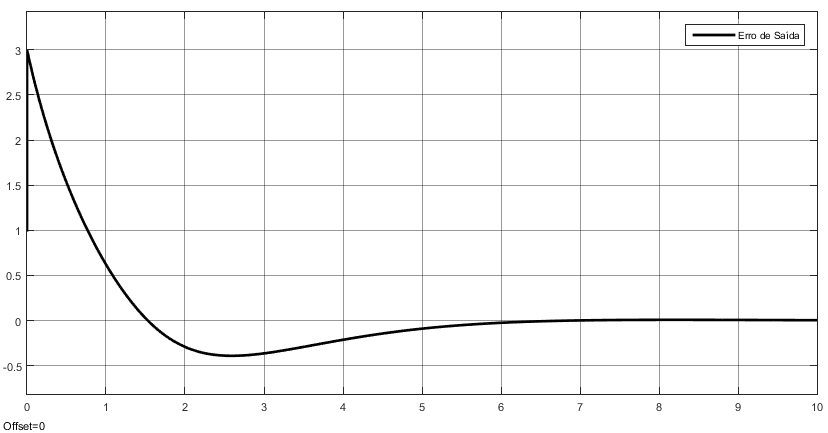
\includegraphics[width = 15 cm, height = 9 cm]{./pics/Erro_de_saida_MRAC_MIT_10seg.png}
 \caption{Erro de Saída da Planta, 10 segundos de simulação}
 \end{figure}

Na figura 1.2, para 10000 segundos de simulação, observamos a convergência das estimativas dos parâmetros da planta no espaço de parâmetros para seus valores corretos, dada uma entrada persistentemente excitante:

\begin{figure}
 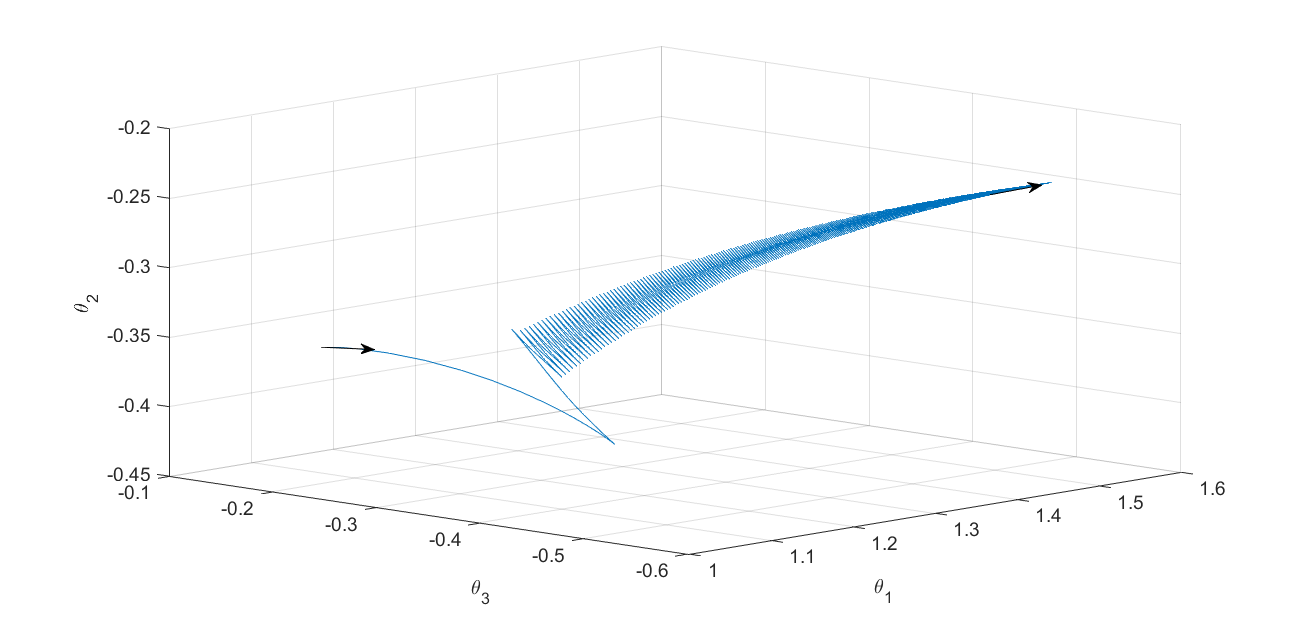
\includegraphics[width = 15 cm, height = 9 cm]{./pics/Trajetoria_MRAC_MIT_10000seg.png}
 \caption{Trajetória das estimativas dos parâmetros da planta, 10000 segundos de simulação}
\end{figure}

\chapter{Método do Gradiente}

Com a mesma planta usada nas simulações anteriores, definimos o erro entre a saída da planta e a estimativa para a saída da planta:

\begin{equation}
\varepsilon = y - \hat{y}
\end{equation}

Onde a estimativa da saída da planta é:

\begin{equation}
\hat{y} = \theta_{c1}\dot{y}_f + \theta_{c2} y_f + \theta_{c3}u_f
\end{equation}

A partir do critério de minimização de custo da função convexa obtemos as leis adaptativas:

\begin{equation}
\dot{\theta}_{c1} = \gamma_1 \varepsilon \dot{y}_f
\end{equation}

\begin{equation}
\dot{\theta}_{c2} = \gamma_2 \varepsilon y_f
\end{equation}

\begin{equation}
\dot{\theta}_{c3} = -\gamma_3 \varepsilon u_f
\end{equation}

E escolhemos $\gamma = [1 1 1]$ novamente.

\chapter*{Introdução}


\section*{Considerações}

Este roteiro de trabalho já foi entregue durante a graduação, para casos particulares de plantas da primeira, segunda e terceira ordem usando os softwares PSIM e Simulink. Estes softwares produzem resultados de simulação através da montagem dos seus diagramas de blocos. Portanto seu uso torna mais fácil a visualização, e faz com que se prestem muito bem ao aprendizado dos conceitos envolvidos no controle adaptativo e identificação de parâmetros.\\

 No trabalho confeccionado para a disciplina do mestrado, nos focamos progressivamente em escrever o código em linha de comando do software MATLAB,  para produzir características de uso que facilitem a pesquisa e comparação de resultados na área. De fato, procuramos imprimir as seguintes características nos códigos:  

\subsection*{Clareza e Comentários}
Seguimos um guia de estilo para garantir a clareza de leitura do código, colocando comentários num número limitado de colunas e usando o separador "$...$"~ quando necessário. Adicionalmente, procuramos usar uma regra de nomeação das variáveis que permite entender mais rapidamente do que se tratam a primeira vista. Tentamos evitar o uso excessivo de laços e estruturas condicionais, empregando-as apenas quando estritamente necessário.


\subsection*{Reusabilidade e Portabilidade}
Os códigos de cada função foram escritos atribuindo um único propósito a cada um deles. Desta forma por exemplo, as funções usadas para plotagem dos gráficos referentes às simulações foram separadas. Garantimos assim que uma única função de plotagem possa ser usada para vários métodos diferentes de identificação ou controle. Similarmente, adotamos estruturas de dados tanto no argumento de entrada das funções quanto no de saída, o que permite mais facilmente que um resultado seja reproduzido e salvo no espaço de trabalho. Estas práticas permitem o reuso e redirecionamento de cada função dos códigos em várias combinações rapidamente. Por estes motivos, os métodos ensinados em sala foram, de forma geral, implementados de forma generalista, aceitando plantas de ordem qualquer.

\chapter{Controle Adaptativo com Acesso à variáveis de Estado}
\section{Modelo de Referência, Regra do MIT}

\subsection{Parâmetros de Simulação}
Escolhemos um modelo de planta de segunda ordem da seguinte forma:
\begin{equation}
G(s) = \frac{b[1]*s + b[0]}{s^2 + a[1]s + a[0]}
\end{equation}

Com $b$ = [11 0] e $a$ = [11 10], de forma que os polos da planta são -1 e -10. O modelo de referência foi escolhido de forma a aumentar o valor em módulo dos polos da planta em 25 porcento e manter o ganho em regime permanente para referência do tipo degrau. De forma que temos o seguinte modelo:

\begin{equation}
G_m(s) = \frac{1.5625b[0]}{s^2 + 1.25a[1]s + 1.5625a[0]}
\end{equation} 

Definimos o erro de saída $e_0$ entre a planta e o modelo de referência, onde $y(t)$ é a saída da planta e $y_m(t)$ a saída do modelo:

\begin{equation}
e_0 = y(t) - y_m(t)
\end{equation}

A partir dos argumentos padrão para controle adaptativo direto, chegamos às leis adaptativas usando a regra do MIT:

\begin{equation}
\dot{\theta}_1 = \gamma_1 e_0 y_f
\end{equation}

\begin{equation}
\dot{\theta}_2 = \gamma_2 e_0 \dot{y}_f
\end{equation}

\begin{equation}
\dot{\theta}_3 = -\gamma_3 e_0 r_f
\end{equation}

Onde o índice $f$ denota a passagem do sinal por um filtro determinado pelo modelo de referência escolhido. Usamos $\gamma_1 = 1$, $\gamma_2=1$ e $\gamma_3=1$, e condições iniciais para a planta e modelo da forma:

\begin{equation}
\theta_m(0) = [0~;~2]
\end{equation}

\begin{equation}
\theta_p(0) = [-4~;~3]
\end{equation}

\subsection{Resultados}

Observamos na Figura 1.1 o erro de saída da planta, para uma referência degrau.\\


 \begin{figure}
 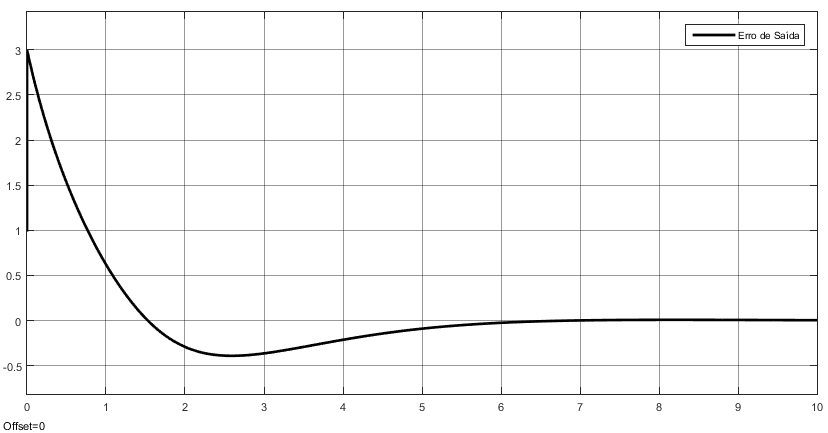
\includegraphics[width = 15 cm, height = 7 cm]{./pics/Erro_de_saida_MRAC_MIT_10seg.png}
 \caption{Erro de Saída da Planta, 10 segundos de simulação}
 \end{figure}

Na Figura 1.2, para 10000 segundos de simulação, observamos a convergência das estimativas dos parâmetros da planta no espaço de parâmetros para seus valores corretos, dada uma entrada persistentemente excitante:

\begin{figure}
 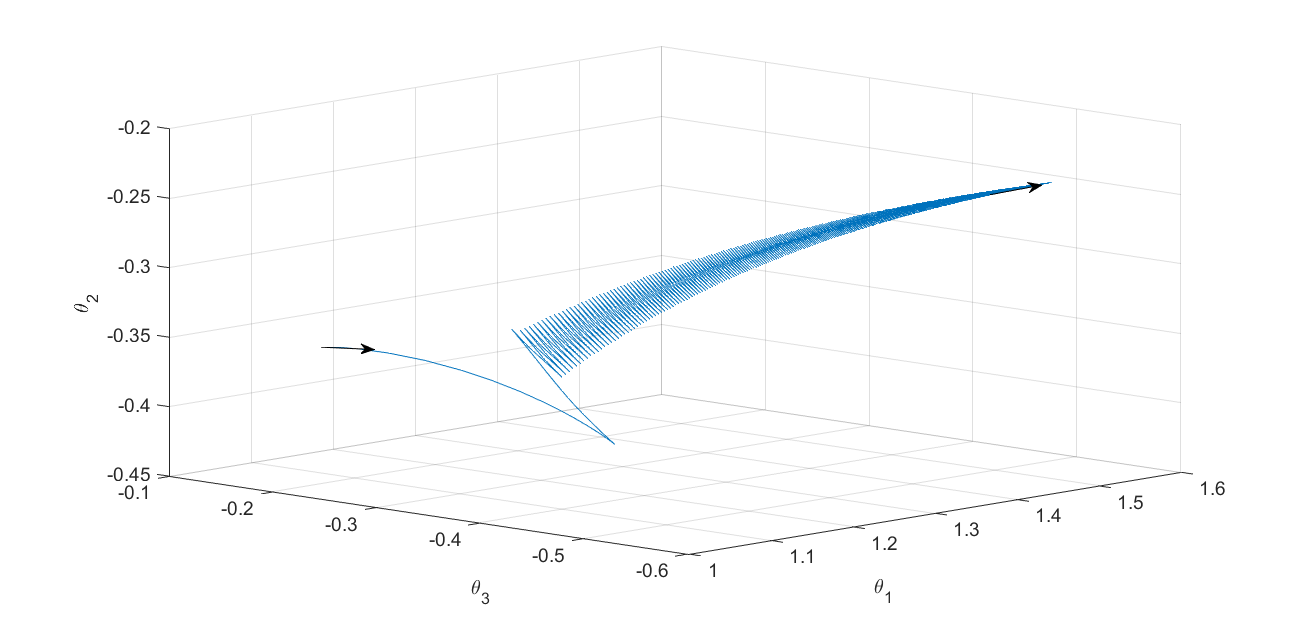
\includegraphics[width = 15 cm, height = 9 cm]{./pics/Trajetoria_MRAC_MIT_10000seg.png}
 \caption{Trajetória das estimativas dos parâmetros da planta, 10000 segundos de simulação}
\end{figure}

\section{Modelo de Referência, Método do Gradiente}

Escolhemos uma planta instável cujos coeficientes do numerador são conhecidos, da forma:

\begin{equation}
G(s) = \frac{1}{s^2+3.6s-2.3}
\end{equation} 

Com o modelo de referência da forma:
\begin{equation}
G_m(s) = \frac{1}{s^2+4s+4}
\end{equation}

Com a planta partindo do repouso e modelo de referência partindo de $[0.2~~0.3]^T$, referência $r(t) = 5+ sen(t) + sen(2*t)$, e matriz de ganhos adaptativos $P = 100*I$. Obtivemos os gráficos da Figura 1.3:

\begin{figure}
 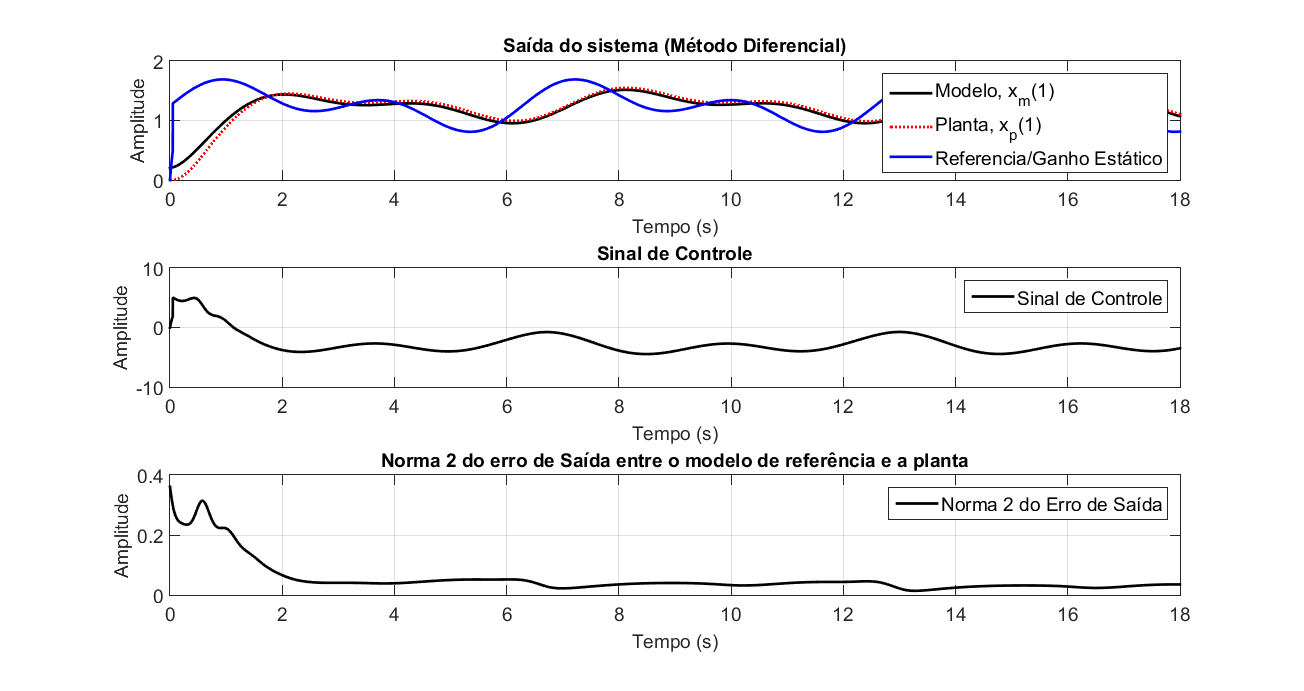
\includegraphics[width = 15 cm, height = 9 cm]{./pics/Figuras_MRACVarEstado.png}
 \caption{a)Saídas do sistema, plotadas contra a referência*ganho estático b)Sinal de Controle c)Norma 2 do erro de saída }
\end{figure}


\chapter{Identificação de Parâmetros}

Neste capítulo, tratamos da tarefa de identificação dos parâmetros da planta escolhida, além de adaptarmos os algoritmos usados para a forma geral mostrada em sala. 

\section{Método do Gradiente Puro}

A planta escolhida para os métodos do gradiente é da forma:

\begin{equation}
G(s) = \frac{1}{s^2 + s + 2}
\end{equation}

O filtro implementado para a obtenção de $z_1$ é da forma:

\begin{equation}
W(s) = \frac{s^2}{s^2+4s+4}
\end{equation}

A referência é um sinal PE da forma:

\begin{equation}
r(t) = 1 +0.3sen(t) + 0.4sen(t)
\end{equation}

A matriz de ganhos adaptativos foi escolhida $\Gamma=30*I$. A matriz de normalização foi deixada como $P'=I$. A planta parte das condições iniciais $[0.2~0.3]$, a estimativa da saída da planta parte do repouso. Escolhemos estimativas iniciais nulas para os parâmetros da planta. Os resultados se encontram na Figura 2.1.

\begin{figure}[htbp!]
 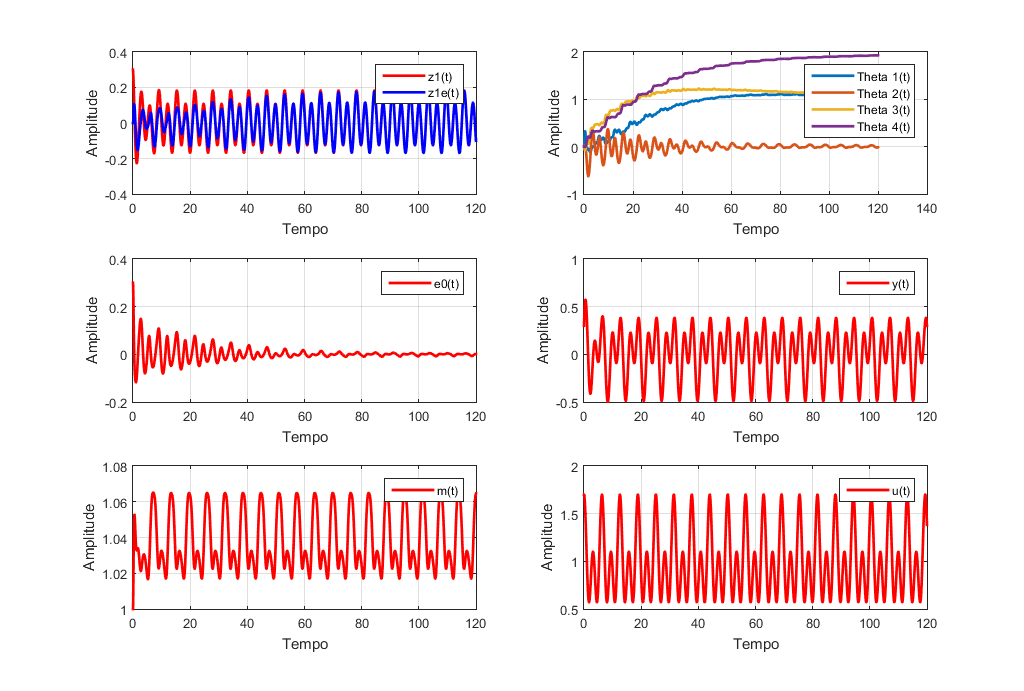
\includegraphics[width = 15 cm, height = 9 cm]{./pics/Figuras_Grad.png}
 \caption{\emph{a)Filtrado e Estimativa do Filtrado b)Estimativas dos parâmetros c)Erro de Saída d) Saída da Plantae)Sinal de Normalização f)Sinal de Controle}}
\end{figure}


\section{Método do Gradiente com Função de Custo Integral}

Implementamos a mesma simulação do caso anterior introduzindo a função de custo integral com $\beta=0.1$. Os resultados se encontram na Figura 2.2.
\begin{figure}[htbp!]
 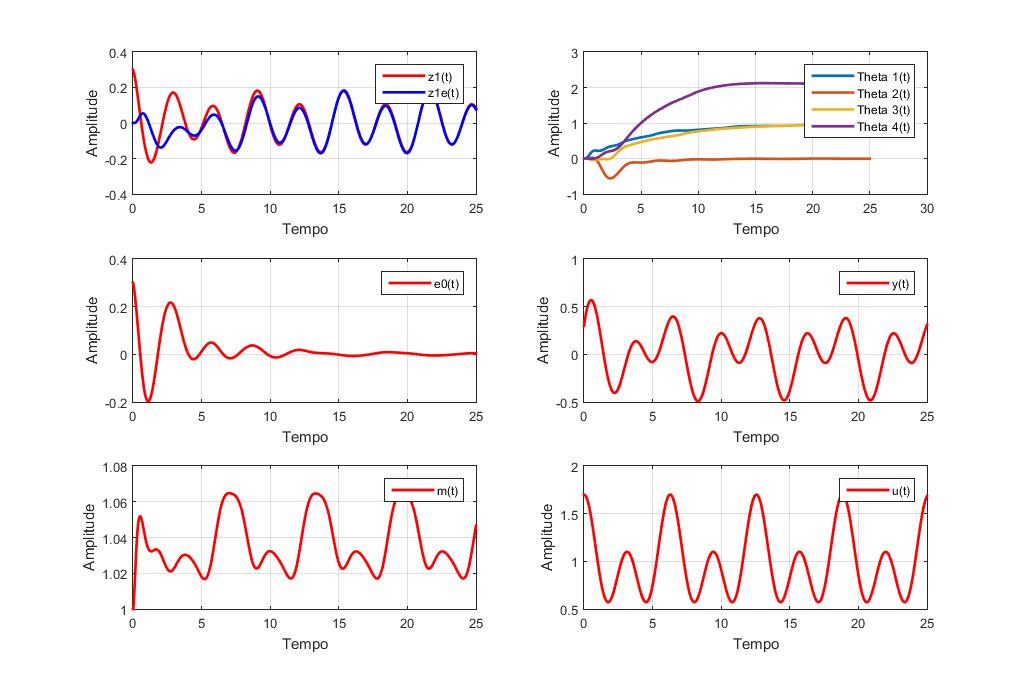
\includegraphics[width = 15 cm, height = 9 cm]{./pics/Figuras_Grad_FCI.png}
 \caption{\emph{a)Filtrado e Estimativa do Filtrado b)Estimativas dos parâmetros c)Erro de Saída d) Saída da Plantae)Sinal de Normalização f)Sinal de Controle}}
\end{figure}

\section{Algoritmo dos Mínimos Quadrados Puro}

A planta escolhida para os métodos dos mínimos quadrados é da forma:

\begin{equation}
G(s) = \frac{-3}{s^2 + 2s + 3}
\end{equation}

A planta parte de $[0.2~0.3]$, a estimativa da saída parte do repouso.Escolhemos as seguintes estimativas iniciais para os parâmetros da planta $\theta_0 =[0~2.1~3.1~1.1]$. Matriz de ganhos adaptativos iniciais $\Gamma_0=100*I$. Matriz de normalização $P'=0.0001*I$. O filtro implementado para a obtenção de $z_1$ é da forma:

\begin{equation}
W(s) = \frac{s^2}{s^2+4s+4}
\end{equation}

A referência é um sinal PE da forma:

\begin{equation}
r(t) = 1 +0.3sen(4*t) + 0.4sen(5*t)
\end{equation}

Observamos os resultados na Figura 2.3.


\begin{figure}[htbp!]
 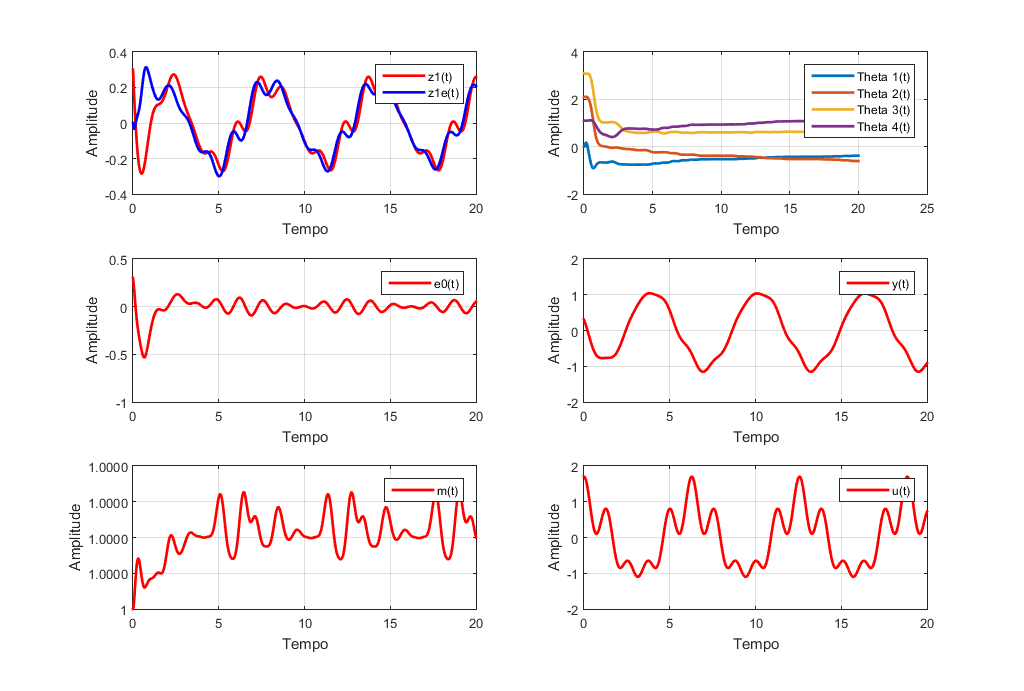
\includegraphics[width = 15 cm, height = 9 cm]{./pics/Figuras_MQ_Puro.png}
 \caption{\emph{a)Filtrado e Estimativa do Filtrado b)Estimativas dos parâmetros c)Erro de Saída d) Saída da Plantae)Sinal de Normalização f)Sinal de Controle}}
\end{figure}

\subsection{Reinicialização de Covariância}

Escolhemos $\lambda_{min}=1$, observamos os resultados da Figura 2.4.

\begin{figure}[htbp!]
 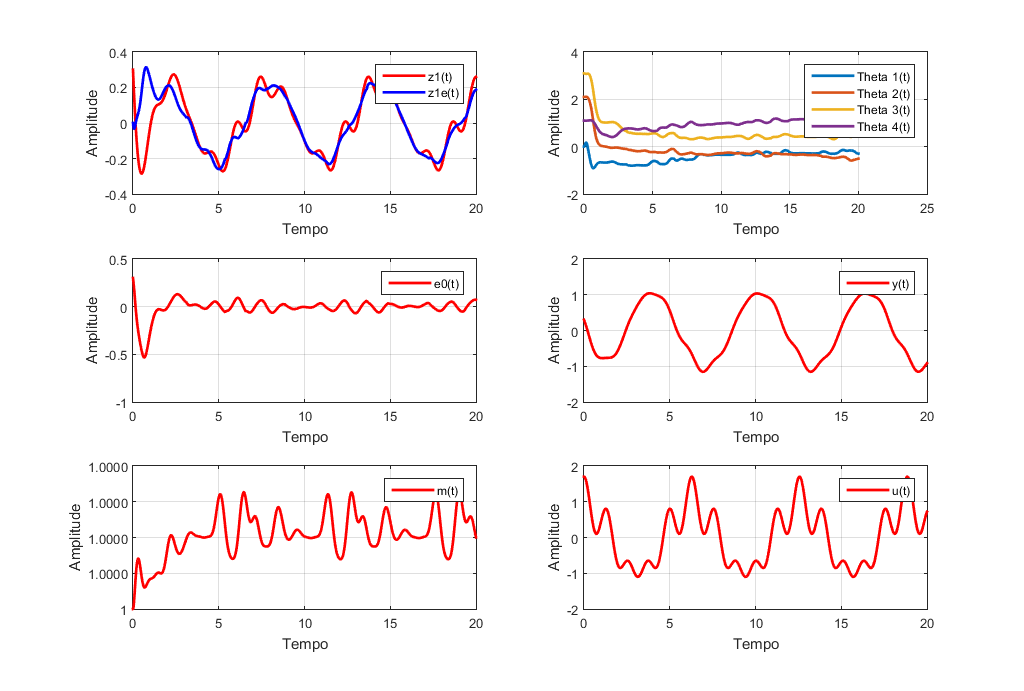
\includegraphics[width = 15 cm, height = 9 cm]{./pics/Figuras_MQ_Puro_RCov.png}
 \caption{\emph{a)Filtrado e Estimativa do Filtrado b)Estimativas dos parâmetros c)Erro de Saída d) Saída da Plantae)Sinal de Normalização f)Sinal de Controle}}
\end{figure}

\section{Algoritmo dos Mínimos Quadrados com Função de Custo Integral}

Escolhemos $\beta=0.5$. Observamos os resultados na figura 2.5.

\begin{figure}[htbp!]
 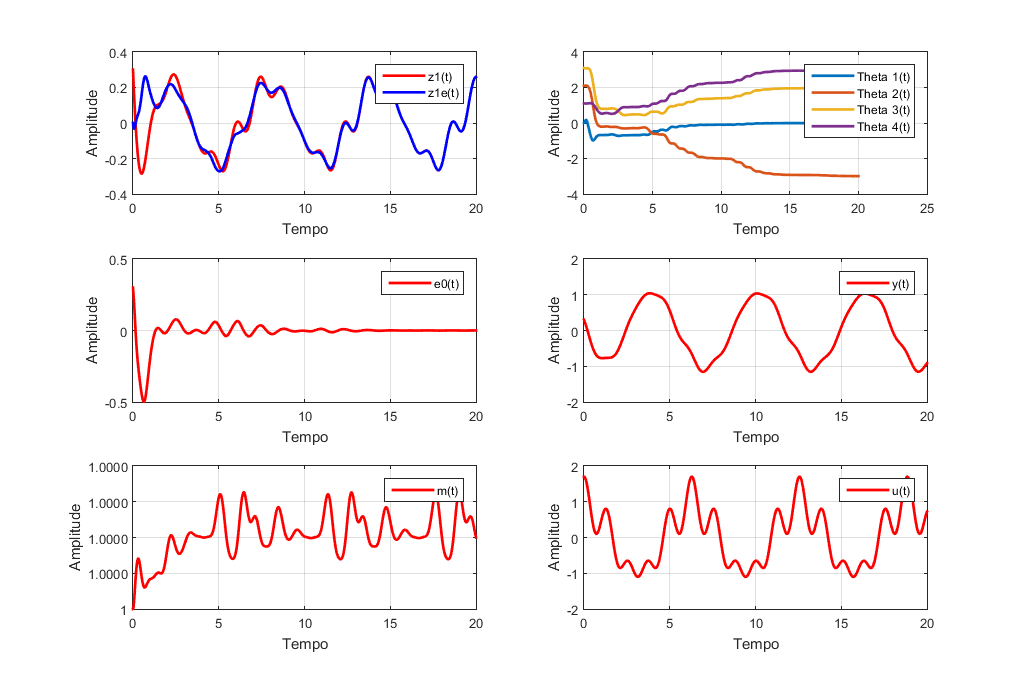
\includegraphics[width = 15 cm, height = 9 cm]{./pics/Figuras_MQ_FE.png}
 \caption{\emph{a)Filtrado e Estimativa do Filtrado b)Estimativas dos parâmetros c)Erro de Saída d) Saída da Plantae)Sinal de Normalização f)Sinal de Controle}}
\end{figure}

\section{Projeção}
Quando a região no espaço de parâmetros em que se encontra o vetor $\theta_p$ da planta é conhecida, uma técnica capaz de favorecer a estabilidade e melhorar o desempenho dos sistemas é de limitar a trajetória das estimativas ao interior da região, fazendo com que, ao chegar na fronteira desta região com tendência de sair, ao invés disso a estimativa seja forçada a deslizar na superfície que delimita a região. Para tanto, é necessário retirar do vetor de adaptação $\dot{\theta}$ sua componente perpendicular à superfície conhecida. Para fazer isto basta conhecer o gradiente da função que delimita a região. 

\section{Referência Degrau}

Os resultados para referência do tipo degrau foram agrupados no final deste capitulo, nas Figuras de 6-10.

\begin{figure}[htbp!]
 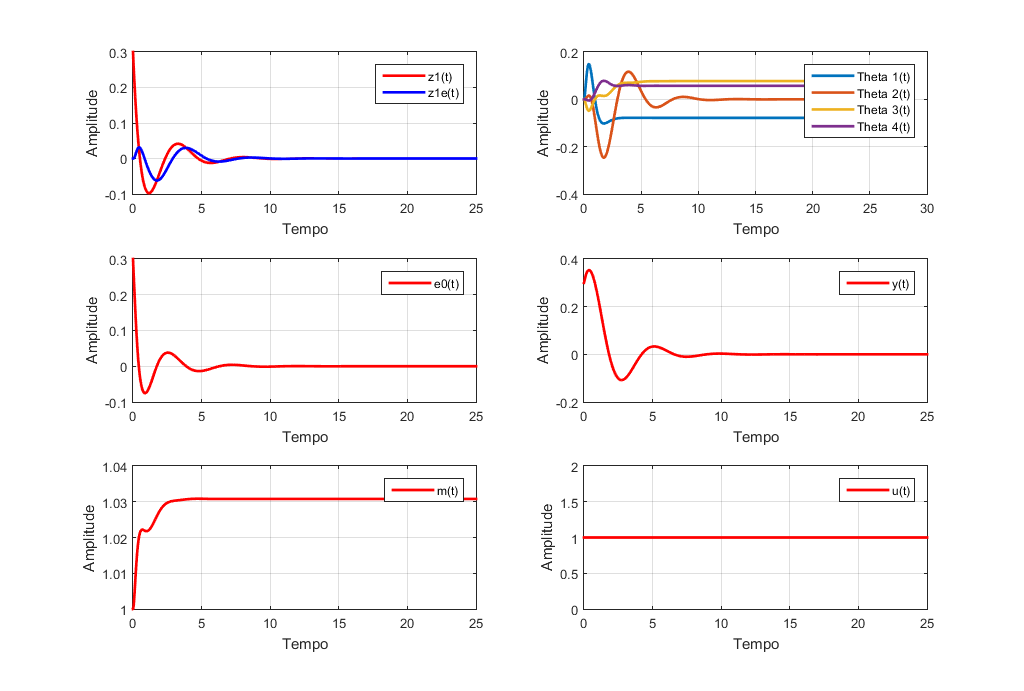
\includegraphics[width = 15 cm, height = 9 cm]{./pics/Figuras_Grad_deg.png}
 \caption{\emph{Gradiente, referência degrau}}
\end{figure}
\begin{figure}[htbp!]
 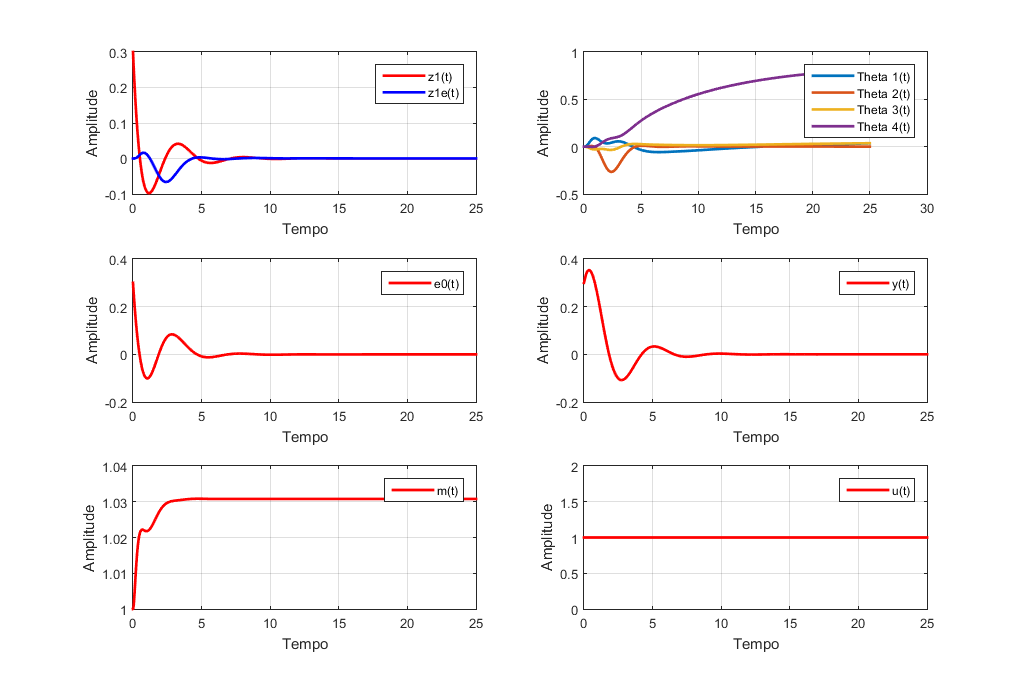
\includegraphics[width = 15 cm, height = 9 cm]{./pics/Figuras_Grad_FCI_deg.png}
 \caption{\emph{Gradiente com função de custo integral, referência degrau}}
\end{figure}
\begin{figure}[htbp!]
 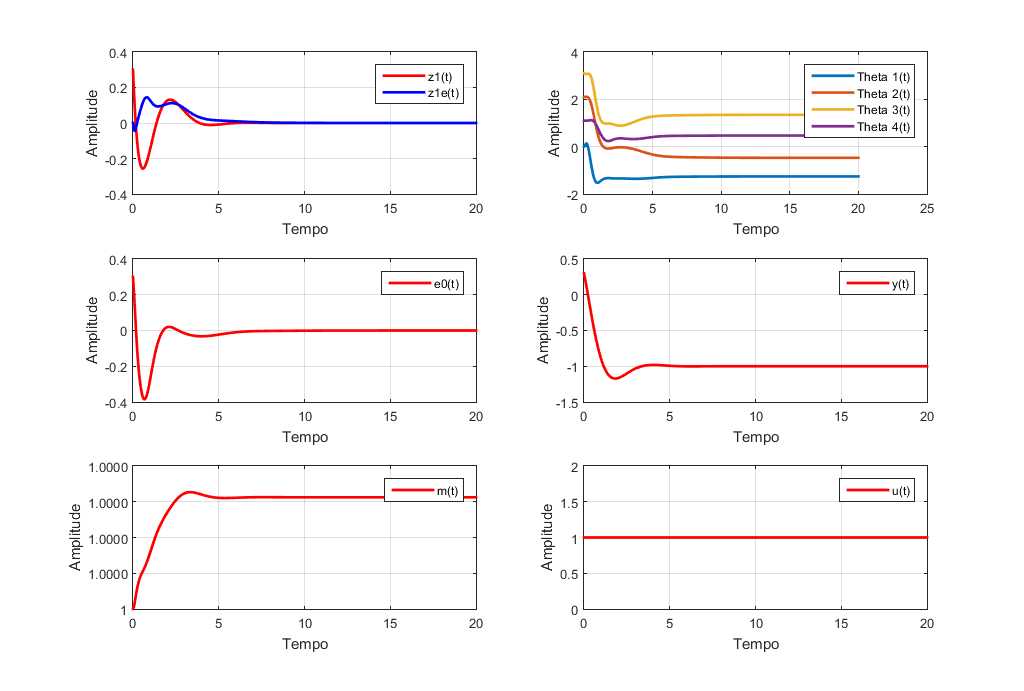
\includegraphics[width = 15 cm, height = 9 cm]{./pics/Figuras_MQ_FE_deg.png}
 \caption{\emph{Mínimos Quadrados com fator de esquecimento, referência degrau}}
\end{figure}
\begin{figure}[htbp!]
 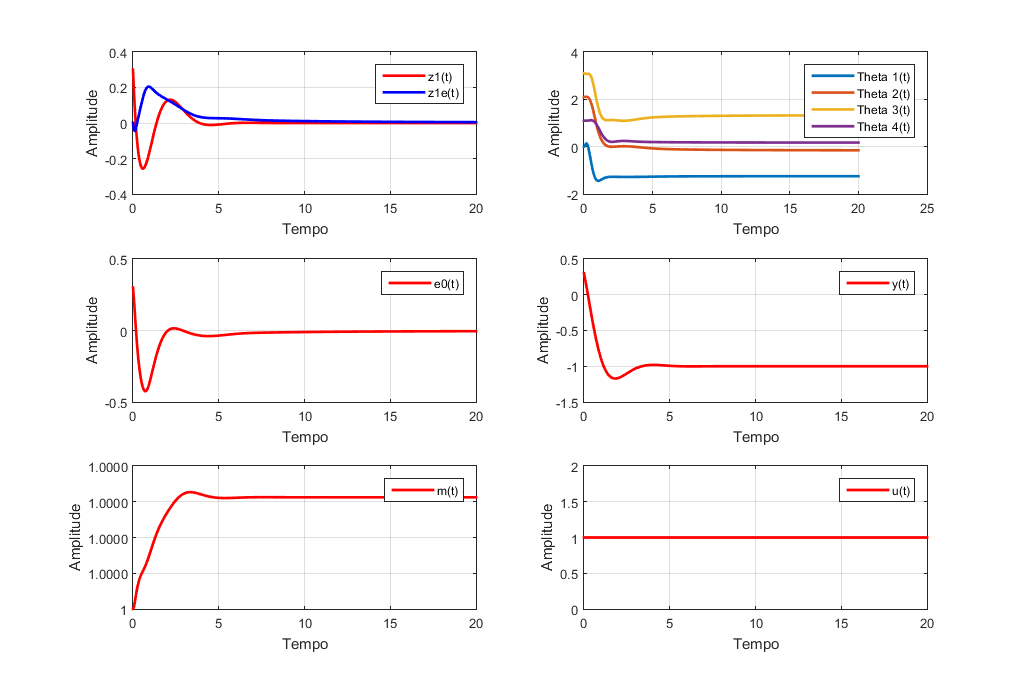
\includegraphics[width = 15 cm, height = 9 cm]{./pics/Figuras_MQ_Puro_deg.png}
 \caption{\emph{Mínimos Quadrados Puro}}
\end{figure}
\begin{figure}[htbp!]
 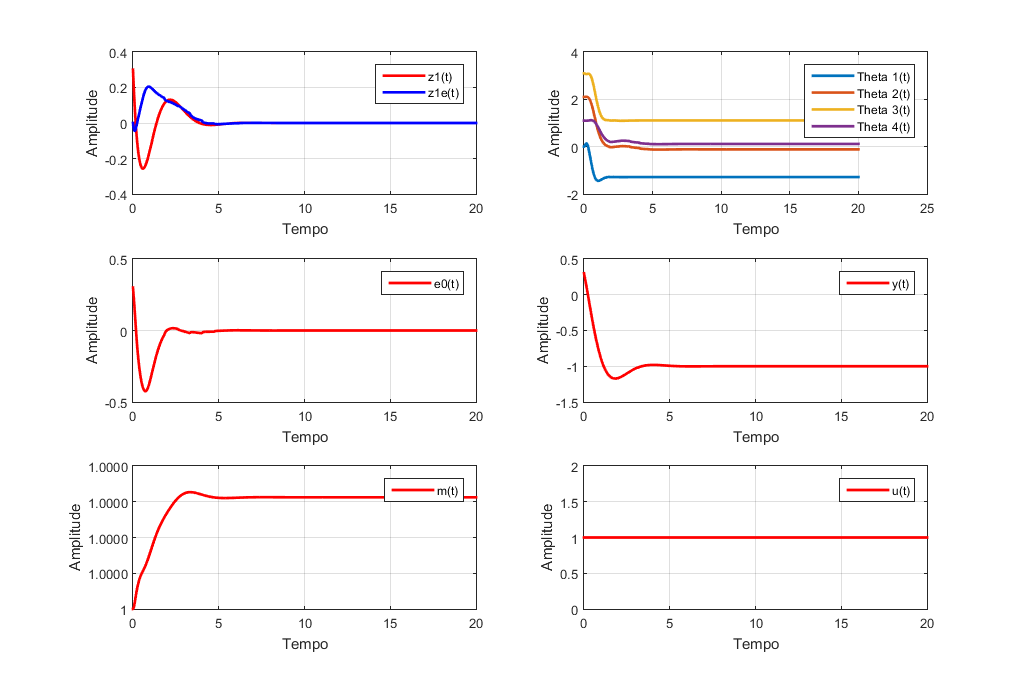
\includegraphics[width = 15 cm, height = 9 cm]{./pics/Figuras_MQ_Puro_RCov_deg.png}
 \caption{\emph{Mínimos Quadrados com Reinicialização de Covariância}}
\end{figure}


\chapter{Controle Adaptativo com Realimentação de Saída}

Até agora, estudamos o controle com acesso às variáveis de estado da planta. Embora sejamos capazes de produzir resultados satisfatórios de posse destas medições, em uma situação prática, estas medidas costumam se provar custosas. É mais fácil do ponto de vista do projetista, por exemplo no controle de um trem, que sejam medidas todas as variáveis relevantes à dinâmica do veículo (e.g.: torque do motor, aceleração, inclinação, momento angular, inercia e velocidade). Porém isto equivaleria ao uso de sensores adaptados para a medida física de cada uma destas variáveis, o que implica em aumento do custo de implementação do sistema.\\

Mais comumente, é feito o controle através de Realimentação de Saída, onde apenas a variável escolhida para ser controlada é medida de fato.\\  

\section{Posicionamento de Polos, Método Polinomial}

Implementamos o controle por Posicionamento de Polos tomando como estratégia para identificação de parâmetros o algoritmo dos mínimos quadrados com fator de esquecimento. O APPC consiste, de forma geral, na resolução da equação diofantina $Qm(s)*\hat{R}(s)*L(s) + \hat{Z}(s)*P(s) = A^*$ para $L(s)$ e $P(s)$, onde $\hat{R}(s)$ e $\hat{Z}(s)$ são estimativas para os polinômios $R(s)$ e $Z(s)$ da planta. Fizemos a implementação do filtro $\Lambda(s)$ de forma a generalizar a implementação. O método usado para a resolução da equação foi através de montagem e inversão da matriz $M_s$ de Sylvester usando os coeficientes dos polinômios conhecidos. Escolhemos esse método apesar de suas várias limitações pois é o mais simples. Embora a adaptação dos parâmetros faça com que ocasionalmente possa acontecer que $det(M_s)\approx0$, evitamos esta situação condicionando o cálculo de $L(s)$ e $P(s)$ a $|det(M_s)|>0.1$, para evitar que os coeficientes de $L(s)$ e $P(s)$ se tornem muito grandes.\\

A planta escolhida é da forma:

\begin{equation}
G(s) = \frac{0.2s + 2}{s^2+3s+4}
\end{equation}

O polinômio de malha fechada desejado é:
\begin{equation}
A^*(s) = \frac{1}{s^4+5.2s^3+12.4s^2+12.6s+6}
\end{equation}

E, como devemos seguir uma referência degrau, o princípio do modelo interno nos dá:
\begin{equation}
Q_m(s) = s 
\end{equation}

Escolhemos as estimativas iniciais dos parâmetros da planta tal que:
\begin{equation}
\hat{R}_0(s) = s^2+2s+5
\end{equation}

\begin{equation}
\hat{Z}_0(s) = 0.1s+3
\end{equation}

Escolhemos um filtro arbitrário, embora seja desnecessário no caso, pois nossa planta é estável. Isto foi feito pois o código foi escrito levando em conta um filtro de ordem adequada para o caso geral, de forma que temos:

\begin{equation}
\Lambda(s) = 2s^2+0.6s+0.7
\end{equation}

Que em princípio, não altera em nada o funcionamento do sistema. Similarmente o sinal de normalização foi mantido, porém com uma matriz $P'$ de norma extremamente pequena.\\



Os resultados da simulação se encontram na figura 3.1.
\begin{figure}
 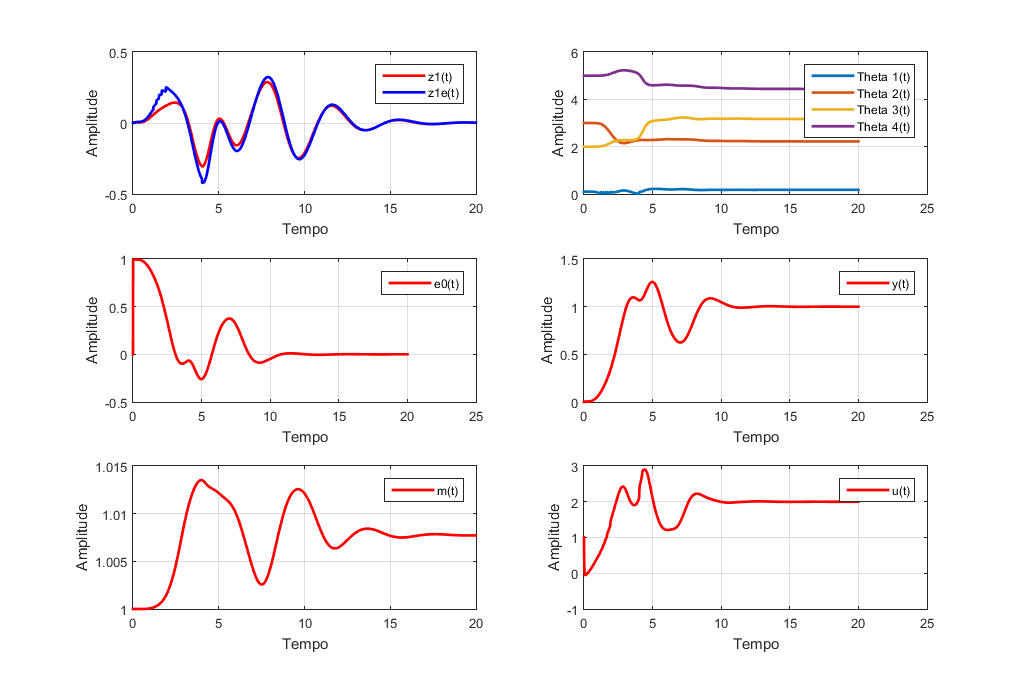
\includegraphics[width = 15 cm, height = 9 cm]{./pics/Figuras_APPC.png}
 \caption{\emph{a)Filtrado da entrada e estimativa do filtrado b)Valores das estimativas dos parâmetros c)Erro de Saída d)Saída da Planta e)Sinal de Normalização} }
\end{figure}


\section{Modelo de Referência}

Implementamos o MRAC para grau relativo $n_r^*>1$, para uma planta de ordem qualquer que necessite do filtro $L(s)$. A planta escolhida para as simulações foi:

\begin{equation}
G(s) = \frac{3}{s^2+3s+3}
\end{equation}

O modelo de referência:

\begin{equation}
G_m(s) = \frac{4}{s^2 +5s+4}
\end{equation}

E o filtro:

\begin{equation}
L(s) = s+1.5
\end{equation}

Com a planta e o modelo partindo do repouso, $\Gamma = I$, $\gamma=10$, estimativas iniciais dos parâmetros $\theta_0 = [1~1~1~2.5]^T$, $\theta_{2n+1}(0)=0.4$, $\alpha=1$. Obtivemos os graficos da Figura 3.2:

\begin{figure}[htbp!]
 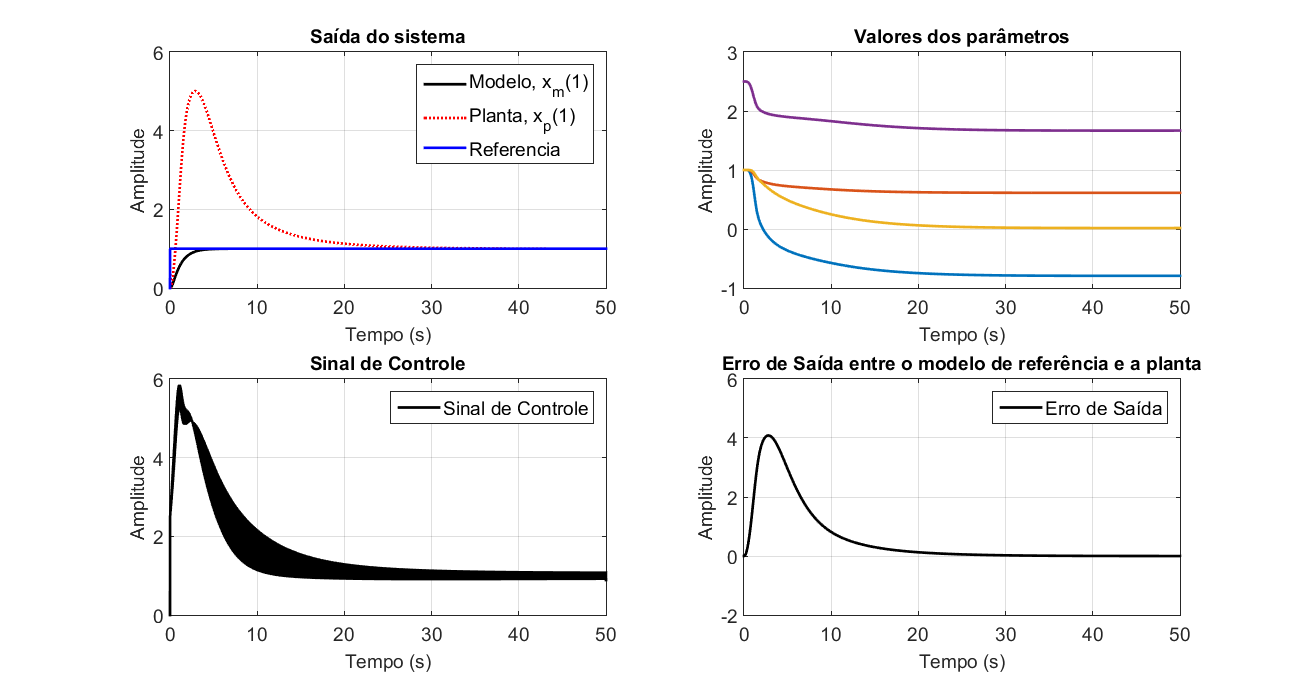
\includegraphics[width = 15 cm, height = 9 cm]{./pics/Figuras_MRAC.png}
 \caption{\emph{a)Saídas do sistema b)Valores das estimativas dos parâmetros c)Sinal de Controle d)Erro de Saída}}
\end{figure}


\section{PID Adaptativo, Método de \"{A}strom-H\"{a}gglund}

O controlador PID Adaptativo é o método de implementação prática mais utilizado. Isso se deve à facilidade com que os parâmetros do controlador são obtidos. Consiste do desligamento do controle quando é observada uma deterioração no comportamento da planta e subsequente substituição do controle por um relé que atua conforme o sinal do erro. A medida que a saída da planta evolui e entra em auto-oscilação, observamos a amplitude e período destas oscilações para sintonizar os parâmetros do controlador via Ziegler-Nichols. O critério escolhido para determinar que houve tal deterioração é estritamente do projetista, pois se trata de uma avaliação subjetiva. De fato, escolhemos para nosso sistema o seguinte critério: houve deterioração se o módulo do erro se manteve acima de 0.3 durante 3 ou mais segundos. A amplitude do relé escolhido é de 5.\\

A planta escolhida tem parâmetros que variam no tempo lentamente e é da forma:

\begin{equation}
G(s) = \frac{1}{s^2 + 2s + cos(0.001*t)+1.1}
\end{equation}

Ao medir $T_{cr}$ e $K_{cr}$, fazemos o cálculo automático dos parâmetros do controlador através da tabela. Os resultados obtidos estão na Figura 3.3.

\begin{figure}[htbp!]
 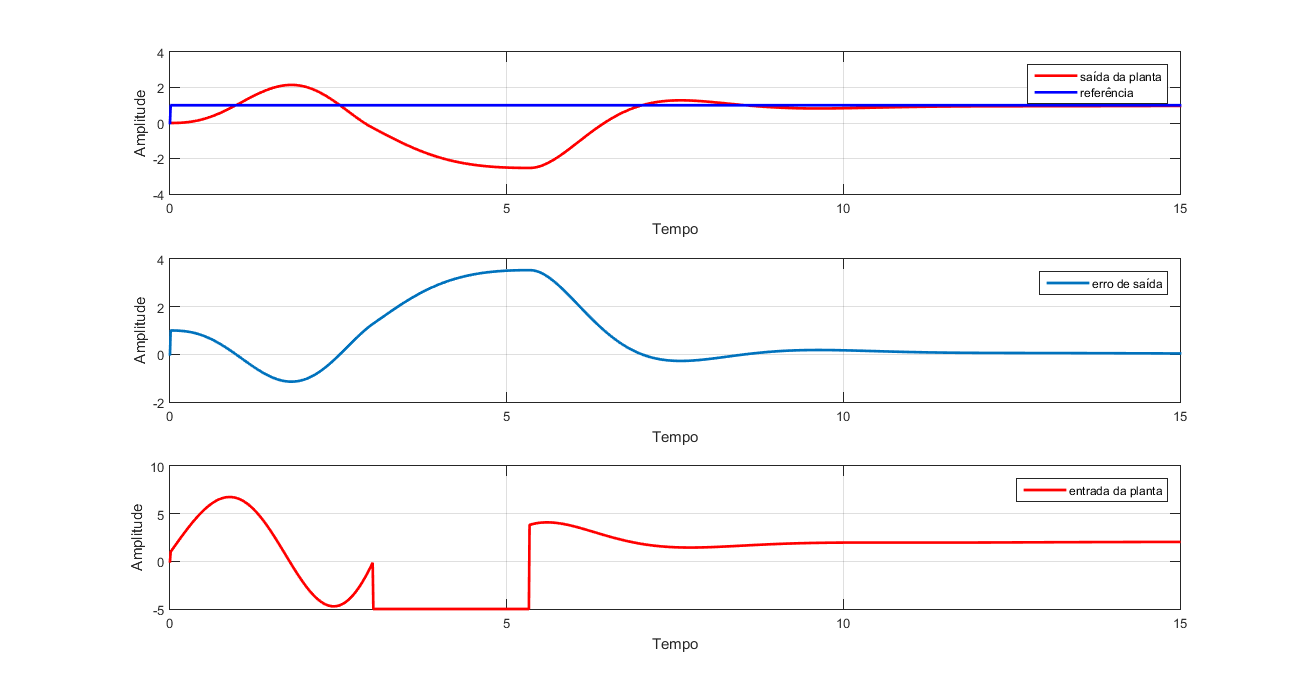
\includegraphics[width = 15 cm, height = 9 cm]{./pics/Figuras_AstHagg.png}
 \caption{\emph{a)Saídas do sistema b)Erro de Saída c)Sinal de Controle}}
\end{figure}

\section{Códigos Comentados}

Tentamos implementar os métodos de forma generalista, para ilustrar colocamos aqui as funções principais de dois dos métodos deste capítulo.

\subsection{APPC}
\begin{verbatim}
%função referente ao controle adaptativo de uma planta de grau qualquer
%usando o método do posicionamento de polos combinado com identificação dos
%parâmetros da planta via método do mínimos quadrados.
%Narendra
%Aluno: Pedro Gushiken
%Orientador: Aldayr Dantas de Araújo

%O argumento da função é uma uma estrutura de dados contendo os polinômios
%da planta, modelo interno, polinômio A* desejado, filtro Lambda, a
%referência expressa como soma de senoides, tempo de simulação, passo de
%integração fixo, condições iniciais, modelos de identificação e parâmetros
%do método de estimação.

%Qm*R*L + Z*P = A_estrela, Qm é conhecido, R e Z são estimados, A_estrela é
%conhecido
function estrutura_de_saida = APPC( estrutura_de_entrada )

[t_inicial,t_final,h, filtroW, ~, ~, ordem, P0,Plinha,cond_inicial_p, ...
cond_inicial_est_p, teta_inicial,Beta,~,~,refF,refA,Qms,Zs_estrela,...
Rs_estrela,A_estrela,Lambda] = convert_struct(estrutura_de_entrada);
[Ap,bp,Cp,Dp] = tf2ss(Zs_estrela, Rs_estrela);
[Aw,bw,Cw,~] = tf2ss([0 filtroW(length(filtroW))],filtroW);
vaux(length(filtroW)) = 0; vaux(1)=1;
[Aw1,bw1,Cw1,Dw1] = tf2ss(vaux,filtroW);
q = length(Qms)-1;
n = length(Rs_estrela)-1;
P(:,:,1) = P0;teta(:,1,1) = teta_inicial;
tempo(1) = t_inicial;
z_est(ordem,1) = 0;
fi1(ordem,1,1) = 0; 
fi2(ordem,1,1) = 0;
x_p_ponto(ordem,1,1) = 0;
u(1) = 1; 
x_p(:,1,1) = cond_inicial_p;
    x_fil1(ordem,1,1) = 0;
    x_fil2(ordem,1,1) = 0;
x_p_ponto(:,1,1) = Ap*x_p(:,1,1) + bp*u(1);
fi(:,1,1) = [fi1(:,1,1);fi2(:,1,1)];
fi(:,1,1)
ns2(1) = transpose(fi(:,1,1))*Plinha*fi(:,1,1);
m(1) = sqrt(1+ns2(1));
teta(:,1,1) = teta_inicial;
z1e(1) = transpose(teta(:,1,1))*fi(:,1,1);
P(:,:,1)=P0;
hlinha(ordem,1) = 1;
h_transposto = transpose(hlinha);
x_p_out(1) = h_transposto(1,:)*x_p(:,1,1);
z1(1) = Cw*z_est(:,1,1) + x_p_out(1);
eo(1) = (z1(1)-z1e(1))/m(1)^2;
l(ordem,1) = 0; l(1,1)=1;
e(1) = 0;
x_fil1_out(1)=0;
x_fil2_out(1)=0;
x_c_out(1)=0;
coefs(2*n+q) = 0.1; 
endk = (t_final-t_inicial)/h;
for k=1:endk
   
tempo(k+1) = tempo(k) + h;
r(k+1) = refA*cos(tempo(k)*refF);
%%%%%%%%%%%%%%%%%%%%%%%%%%%%%%
%algoritmo de estimação
%Filtragem de y(t)
z_est_ponto(:,1,k) = Aw1*z_est(:,1,k) + bw1*x_p_out(k);
z_est(:,1,k+1) = z_est(:,1,k) + h*z_est_ponto(:,1,k);
z1(k) = Cw1*z_est(:,1,k) + Dw1*x_p_out(k);

%%%%%%%%%%%%%%%%%%%%%%%%%%%%%%%%%%%%

%Geração do Vetor fi;
fi1_p(:,1,k) = Aw*fi1(:,1,k) + bw*u(k);
fi1(:,1,k+1) = fi1(:,1,k) + h*fi1_p(:,1,k);
fi2_p(:,1,k) = Aw*fi2(:,1,k) + bw*x_p_out(k);
fi2(:,1,k+1) = fi2(:,1,k) + h*fi2_p(:,1,k);
fi(:,1,k) = [fi1(:,1,k);-fi2(:,1,k)];


%sinal de normalização
ns2(k) = transpose(fi(:,1,k))*Plinha*fi(:,1,k);
m(k) = sqrt(1+ns2(k));

%Cálculo da matriz de ganhos adaptativos P
P_ponto(:,:,k) = Beta*P(:,:,k)-P(:,:,k)*fi(:,1,k)*transpose(fi(:,1,k))*P(:,:,k)/m(k)^2;
P(:,:,k+1) = P(:,:,k) + h*P_ponto(:,:,k);


%lei adaptativa
z1e(k) = transpose(teta(:,1,k))*fi(:,1,k);
eo(k) = (z1(k)-z1e(k))/m(k)^2;
teta_p(:,1,k) = P(:,:,k)*eo(k)*fi(:,1,k);

teta(:,1,k+1) = teta(:,1,k) + h*teta_p(:,1,k);
    for j=1:2*n
       if teta(j,1,k+1)<0
          teta(j,1,k+1)=0.1;
       end
    end

Zs_chapeu(:,1) = teta(1:n,1,k+1);
Rs_chapeu(:,1) = [1;teta(n+1:2*n,1,k+1)];


%fim do algoritmo de estimação
%APPC
    QmRs=conv(Qms,Rs_chapeu);
    M = M_sylv(n,q,QmRs,Zs_chapeu);
    if abs(det(M))>=0.1
    coefs = ((M^-1)*A_estrela)';
    end
    Ls = coefs(1:n);
    Ps = coefs(n+1:2*n+q);
    for j=1:n
       if Ls(n)<0
          Ls(n)=0;
       end
    end
    for i=1:n+q
        if Ps(i)<0
            Ps(i)=0;
        end
    end

    
    [Afil1,bfil1,Cfil1,Dfil1] = tf2ss((Ps),(Lambda)');
    [Afil2,bfil2,Cfil2,Dfil2] = tf2ss((Lambda'-conv(Qms,Ls)),(Lambda)');

    x_fil1_ponto(:,1,k) = Afil1*x_fil1(:,1,k) + bfil1*e(k);
    x_fil1(:,1,k+1) = x_fil1(:,1,k)+h*x_fil1_ponto(:,1,k);
    x_fil1_out(k+1) = Cfil1*x_fil1(:,1,k+1) + Dfil1*x_fil1_out(k);
    
    x_fil2_ponto(:,1,k) = Afil2*x_fil2(:,1,k) + bfil2*u(k);
    x_fil2(:,1,k+1) = x_fil2(:,1,k)+h*x_fil2_ponto(:,1,k);
    x_fil2_out(k+1) = Cfil2*x_fil2(:,1,k+1) + Dfil2*u(k);
    
    u(k+1) = x_fil2_out(k+1) + x_fil1_out(k+1);
    
    x_p_ponto(:,1,k) = Ap*x_p(:,1,k) + bp*u(k);
    x_p(:,1,k+1) = x_p(:,1,k)+h*x_p_ponto(:,1,k);
    x_p_out(k+1) = Cp*x_p(:,1,k+1) + Dp*u(k);
    
    e(k+1) = r(k+1) - x_p_out(k+1);
    
end
estrutura_de_saida = make_struct_out                        ...
        (teta, tempo, z1, z1e, e, x_p_out,m,u);


end
\end{verbatim}


\subsection{MRAC}

\begin{verbatim}
function Estr_Dados_saida = MRAC_NRQ(Estr_Dados_Entrada)
%MRAC_NRQ, retorna uma estrutura de dados contendo resultados da simulação
%de um sistema de controle adaptativo por modelo de referência para uma
%planta de grau relativo qualquer dado como argumento uma estrutura de
%dados contendo os filtros, planta, referência expressa como soma de
%senoides, tempo de simulação, passo de integração fixo, condições iniciais
%e estimativas iniciais dos parâmetros, além dos ganhos adaptativos da matriz
%P(=Gamma) e do escalar gamma.


%algoritmo de conversão da  estrutura de dados colocada no argumento
[stoptime, h, filtroL, filtroM_num, filtroM_den, planta_numerador,  ...
 planta_denominador,cond_iniciais_p,cond_iniciais_m,referenciaEps,  ...   
 referenciaF,P,gamma,est_theta_inic,theta_2nm1_0,alfa,kp,km]                                ...
 = convert_struct(Estr_Dados_Entrada);

%número de passos da simulação
endk = floor(stoptime/h);

%matrizes relacionadas à planta, ~ representa uma variável cujo valor não
%importa e portanto não precisa ser assinalado, no caso a matriz D_p da
%planta que é sempre 0 pois a planta deve ter grau relativo pelo menos 1
[A_p,b_p,C_p,~] = tf2ss(kp*planta_numerador,planta_denominador);

%matrizes relacionadas aos filtros M(s) e L(s)
    %Matrizes de M(s)*L(s)
    [A_ML,b_ML,C_ML,D_ML] = tf2ss(km*filtroM_num.*filtroL,filtroM_den);
    %Matrizes de M(s)
    [A_M,b_M,C_M,D_M] = tf2ss(km*filtroM_num,filtroM_den);
    %Matrizes de L^-1(s)
    [A_Lm1,b_Lm1,C_Lm1,D_Lm1] = tf2ss(1,filtroL);
%Matriz canônica de LAMBDA, tal que det(sI-Lambda) = numerador de M(s)
     Lambda = can(fliplr(-filtroM_num));
    
%ordem da planta
n = length(planta_denominador) - 1;

%condições iniciais dos parâmetros
theta(:,1,1) = est_theta_inic;
x_p(:,1,1) = cond_iniciais_p;
x_m(:,1,1) = cond_iniciais_m;
u(1) = 0;
v_1(:,1,1) = zeros(n-1,1);
v_2(:,1,1) = zeros(n-1,1);
g(n-1,1) = 1;
L1tw(:,1,1) = zeros(n-1,1); 
tempo(endk) = 0;
tL1w_d(n-1,2*n,1) = 0;
theta_2nm1(1) = theta_2nm1_0;
e_a(1) = 0;
y_aumentado_interno(n,1,1) = 0;
for k=1:endk
    %tempo de simulação
   tempo(k+1) = tempo(k) + h;
   
   %sinal referência, tal que r(t) = a1*sin(f1*t)+...+an*sin(fn*t), onde os
   %vetores referenciaEps e referenciaF são respectivamente vetores linha e
   %coluna de mesmo tamanho. 
   r(k+1) = referenciaEps*cos(tempo(k)*referenciaF);
   
   %equações de espaço de estado do modelo de referência
   x_m_ponto(:,1,k) = A_M*x_m(:,1,k) + b_M*r(k);
   x_m(:,1,k+1) = x_m(:,1,k) + h*x_m_ponto(:,1,k);
   x_m_out(k+1) = C_M*x_m(:,1,k) + D_M*r(k);
   
   %equações de estado da planta
   x_p_ponto(:,1,k) = A_p*x_p(:,1,k) + b_p*u(k);
   x_p(:,1,k+1) = x_p(:,1,k) + h*x_p_ponto(:,1,k);
   x_p_out(k+1) = C_p*x_p(:,1,k+1);
   
   %geração dos filtrados da planta e do sinal de entrada
   v_1_ponto(:,1,k) = Lambda*v_1(:,1,k) + g*u(k);
   v_1(:,1,k+1) = v_1(:,1,k) + h*v_1_ponto(:,1,k);
   v_2_ponto(:,1,k) = Lambda*v_2(:,1,k) + g*x_p_out(k);
   v_2(:,1,k+1) = v_2(:,1,k) + h*v_2_ponto(:,1,k);
   
   %montagem do vetor w
   w(:,1,k+1) = [v_1(:,1,k+1); x_p(k+1); v_2(:,1,k+1); r(k+1)];
   
   %Geração de ya, sinal de saída aumentado, através de suas sub variáveis
   %devido ao fato de haver vários filtros encadeados, para implementar a
   %equação é necessário calcular suas parcelas separadamente em espaço de
   %estados
   
   %parcela = L^-1*theta_transposto*w
   L1tw_ponto(:,1,k) = A_Lm1*L1tw(:,1,k) + b_Lm1*        ...
                       transpose(theta(:,1,k))*w(:,1,k);
   L1tw(:,1,k+1) = L1tw(:,1,k) + h*L1tw_ponto(:,1,k);
   L1tw_out(k+1) = C_Lm1*L1tw(:,1,k+1)+                  ...
                   D_Lm1*transpose(theta(:,1,k))*w(:,1,k);
   
   %parcela = L^-1*w
   for d=1:length(w(:,1,k))
       tL1w_d_ponto(:,d,k) = A_Lm1*tL1w_d(:,d,k) + b_Lm1*w(d,1,k);
       tL1w_d(:,d,k+1) = tL1w_d(:,d,k) + h*tL1w_d_ponto(:,d,k);
       tL1w(d,1,k+1) = C_Lm1*tL1w_d(:,d,k+1)+D_Lm1*w(d,1,k);
   end
   
   %parcela = (L^-1*w) transposto * (L^-1*w)
   
   L1wTL1w(k+1) = transpose(tL1w(:,1,k+1))*tL1w(:,1,k+1);
   
   %parcela interna de y_aumentado:
   p_int(k+1) =                                                           ...
   theta_2nm1(k)*(L1tw_out(k+1)-transpose(theta(:,1,k))*tL1w(:,1,k+1))    ...
   +alfa*e_a(k)*L1wTL1w(k+1);
   
   %geração de y aumentado em espaço de estados
   y_aumentado_ponto(:,1,k) = A_ML*y_aumentado_interno(:,1,k) + b_ML*p_int(k);
   y_aumentado_interno(:,1,k+1) = y_aumentado_interno(:,1,k) + ...
                                  h*y_aumentado_ponto(:,1,k);
   y_aumentado(k+1) = C_ML*y_aumentado_interno(:,1,k+1) + D_ML*p_int(k+1);
   
   %erro de saída
   e_o(k) = x_p_out(k) - x_m_out(k);
   
   %erro de saída aumentado através da predição
   e_a(k+1) = e_o(k) - y_aumentado(k);
   
   %geração da lei adaptativa para os parâmetros do controlador
   theta_ponto(:,1,k) = -P*e_a(k)*tL1w(:,1,k);
   %atualização dos parâmetros
   theta(:,1,k+1) = theta(:,1,k) + h*theta_ponto(:,1,k);
   
   %geração da lei adaptativa adicional para theta_(2n+1)
   theta_2nm1_ponto(k) = gamma*e_a(k+1)*(L1tw_out(k+1) -           ...
                         transpose(theta(:,1,k))*tL1w(:,1,k+1)); ...
   %atualização do parâmetro theta_(2n+1)
   theta_2nm1(k+1) = theta_2nm1(k)+h*theta_2nm1_ponto(k);
                
   %lei de controle
   u(k+1) = transpose(theta(:,1,k+1))*w(:,1,k+1);
    
end
Estr_Dados_saida = make_struct_out_MRAC(x_p_out,x_m_out,theta,e_o, ...
                                 u, r,tempo,endk);
end

\end{verbatim}


\chapter*{Conclusão}

Implementamos a maior parte das tarefas pedidas na disciplina, buscando melhorar o trabalho feito na graduação em termos de uma abordagem mais generalista dos problemas, voltada para o uso da programação em linha de código. A limitação prévia do aluno neste quesito foi superada. Assim, podemos afirmar que a opção entre o uso dos softwares de simulação por diagrama de blocos ou por linha de comando se trata realmente de uma opção e escolheremos um ou outro por conveniência a partir de agora. Os métodos estudados provém uma boa base para o estudo do Controle Adaptativo e sua implementação em termos de pesquisa, e a nova abordagem permite um uso e comparação mais rápido de resultados.  

\end{document}         